\documentclass[11pt]{article}
\usepackage[margin=1in]{geometry}
\usepackage{graphicx}
\usepackage{booktabs}
\usepackage{hyperref}
\usepackage{amsmath}
\usepackage{caption}
\usepackage{subcaption}
\usepackage{float}
\usepackage{parskip}

\title{Octopus CXL Memory Pooling: Trace Data Exploration}
\author{Pulak Mehrotra}
\date{\today}

\begin{document}
\maketitle
\tableofcontents
\newpage

% =========================================================================
\section{Overview}

This document records the data exploration and diagnostic experiments
conducted on the Azure VM traces used to train the Octopus CXL memory
pooling RL agent. The goal is to understand the structure of the raw
data before designing a data augmentation pipeline.

All experiments use ten production Azure VM traces collected over an
approximately 8-day window in November--December 2023, stored as
pre-processed pickle files in \texttt{data/traces/}. Each pickle
unpacks to a tuple
\texttt{(all\_vms, node\_to\_vms, node\_to\_machine, vm\_type\_sz,
machine\_sz)} where each VM is an instance of the \texttt{VM} class
defined in \texttt{octopus/data.py}.

% =========================================================================
\section{Data Loading and VM Schema}

\subsection{VM Class Fields}

Each VM record contains the following fields relevant to the
simulation:

\begin{center}
\begin{tabular}{lll}
\toprule
Field & Type & Description \\
\midrule
\texttt{rss[1]} & float (MB) & Memory allocation size — \textbf{the only field read by the env} \\
\texttt{start\_time} & datetime & VM arrival time \\
\texttt{end\_time} & datetime & VM termination time \\
\texttt{max\_mem\_ts} & list of [datetime, float] & Per-tick memory utilisation (\%) \\
\texttt{avg\_mem\_ts} & list of [datetime, float] & Per-tick average memory utilisation (\%) \\
\texttt{rss[0]} & float & CPU-related resource (not used by env) \\
\texttt{rss[2]} & float & Storage resource (not used by env) \\
\texttt{rss[3]} & float & Network/IOPS resource (not used by env) \\
\bottomrule
\end{tabular}
\end{center}

The environment (\texttt{octopus/env.py}) reads exactly one field per
VM: \texttt{rss[1]}, the static memory allocation size. The time
series fields \texttt{max\_mem\_ts} and \texttt{avg\_mem\_ts} are never
consumed. Values in those time series are utilisation percentages
(observed values of 43--44 against an \texttt{rss[1]} of 7168\,MB),
so actual consumed memory at tick $t$ would be
$\texttt{rss[1]} \times \texttt{avg\_mem\_ts}[t] / 100$. This richer
signal is ignored in the current implementation.

\subsection{Machine and VM Type Sizes}

\texttt{machine\_sz} maps machine type $\to$ a list of four resource
capacities indexed identically to \texttt{rss}. Index 1 is physical
DRAM. In the AMS20 trace there are four machine types, all with
identical capacity vectors \texttt{[40000, 458812, 5494272,
40000000]}, meaning all nodes have 458\,GB of physical DRAM.
\texttt{vm\_type\_sz} has a similar layout for VM SKUs.

% =========================================================================
\section{Trace Inventory}

Ten traces are available, all spanning approximately the same 8-day
window (2023-11-20 to 2023-11-28):

\begin{center}
\begin{tabular}{llr}
\toprule
Trace & Location & Total VMs \\
\midrule
AMS20PrdApp19-tround.sqlite & Amsterdam & 34,029 \\
BLAPrdApp19-troundgrt5m.sqlite & Bangalore & 129,698 \\
BN9PrdApp18-troundgrt5m.sqlite & BN9 & 178,224 \\
DSM08PrdApp05-troundgrt5m.sqlite & Des Moines & 103,847 \\
DUB24PrdApp09-troundgrt5m.sqlite & Dublin & 79,151 \\
LON23PrdApp01-troundgrt5m.sqlite & London & 23,450 \\
LVL01PrdApp05-troundgrt5m.sqlite & Louisville & 271,080 \\
SG2PrdApp35-troundgrt5m.sqlite & Singapore & 141,018 \\
SYD21PrdApp07-troundgrt5m.sqlite & Sydney & 57,501 \\
YTO21PrdApp05-troundgrt5m.sqlite & Toronto & 80,280 \\
\bottomrule
\end{tabular}
\end{center}

% =========================================================================
\section{The Environment and Simulation Model}

\subsection{Key Concepts}

\textbf{Node.} A physical server in the datacenter. Each node hosts
some set of VMs and has a physical DRAM capacity from
\texttt{machine\_sz}.

\textbf{Pod.} A randomly selected subset of \texttt{pod\_size} nodes
(default: 16) that share CXL memory for one training episode. Pods
are re-sampled every episode by shuffling the node list with a
seed derived from the episode count.

\textbf{Event.} One VM arrival that requires an agent allocation
decision. Each event is a tuple
\texttt{(arrival\_tick, host\_id, rss[1], dealloc\_tick)}.
The number of events per episode equals the number of VMs on the
selected pod nodes that survive the HOTFIX filter.

\subsection{The HOTFIX Filter}

\texttt{\_build\_events} in \texttt{env.py} runs a greedy sequential
filter over each node before building the event list. VMs are
processed in arrival order; if adding a VM would push the node's
running memory total above \texttt{machine\_sz[node\_type][1]},
the VM is added to \texttt{vmkey\_to\_skip} and excluded from the
episode. This enforces physical DRAM feasibility. VMs with
\texttt{vm\_e < 0} (end tick before pod window start) are also
skipped.

\subsection{Reward}

At each VM arrival the reward is:
\[
r = -\frac{\Delta \max_j c_j}{\text{fair\_share}} - \lambda \cdot
\mathrm{Var}\!\left(\frac{c}{\text{fair\_share}}\right)
\]
where $c_j$ is the current load on MPD $j$,
$\text{fair\_share} = \text{pod\_dram} / \text{num\_mhd}$,
and $\lambda = 0.5$ is the variance penalty weight.

% =========================================================================
\section{rss[1] Distribution (Fig 1)}

\begin{figure}[H]
  \centering
  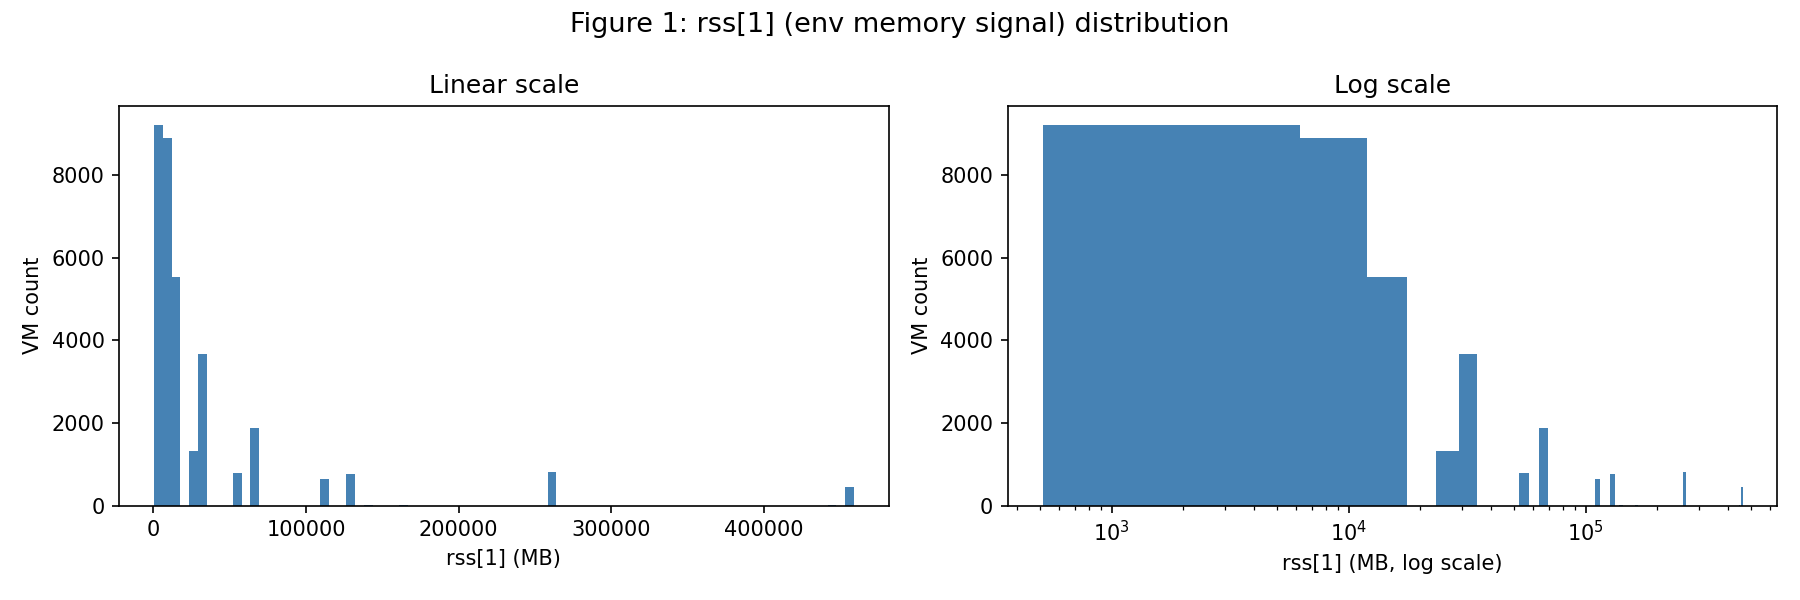
\includegraphics[width=\textwidth]{fig1_rss1_distribution.png}
  \caption{Distribution of \texttt{rss[1]} across all VMs in the AMS20
  trace. Left: linear scale. Right: log scale. Summary statistics:
  min=512\,MB, p5=2048\,MB, p50=8192\,MB, p95=131072\,MB,
  max=458812\,MB.}
\end{figure}

\texttt{rss[1]} is strongly discrete, clustering at powers of two
(512, 1024, 2048, 4096, 8192\,MB, \ldots) because Azure VMs are
provisioned in standard SKU sizes. This has a direct implication for
augmentation: per-VM scaling would destroy the SKU boundaries,
creating memory sizes that do not exist in production.
\textbf{Augmentation must therefore operate at the episode level}
(a single scale factor applied uniformly to all VMs in one episode),
not per-VM.

% =========================================================================
\section{VM Lifetime Distribution (Fig 2)}

\begin{figure}[H]
  \centering
  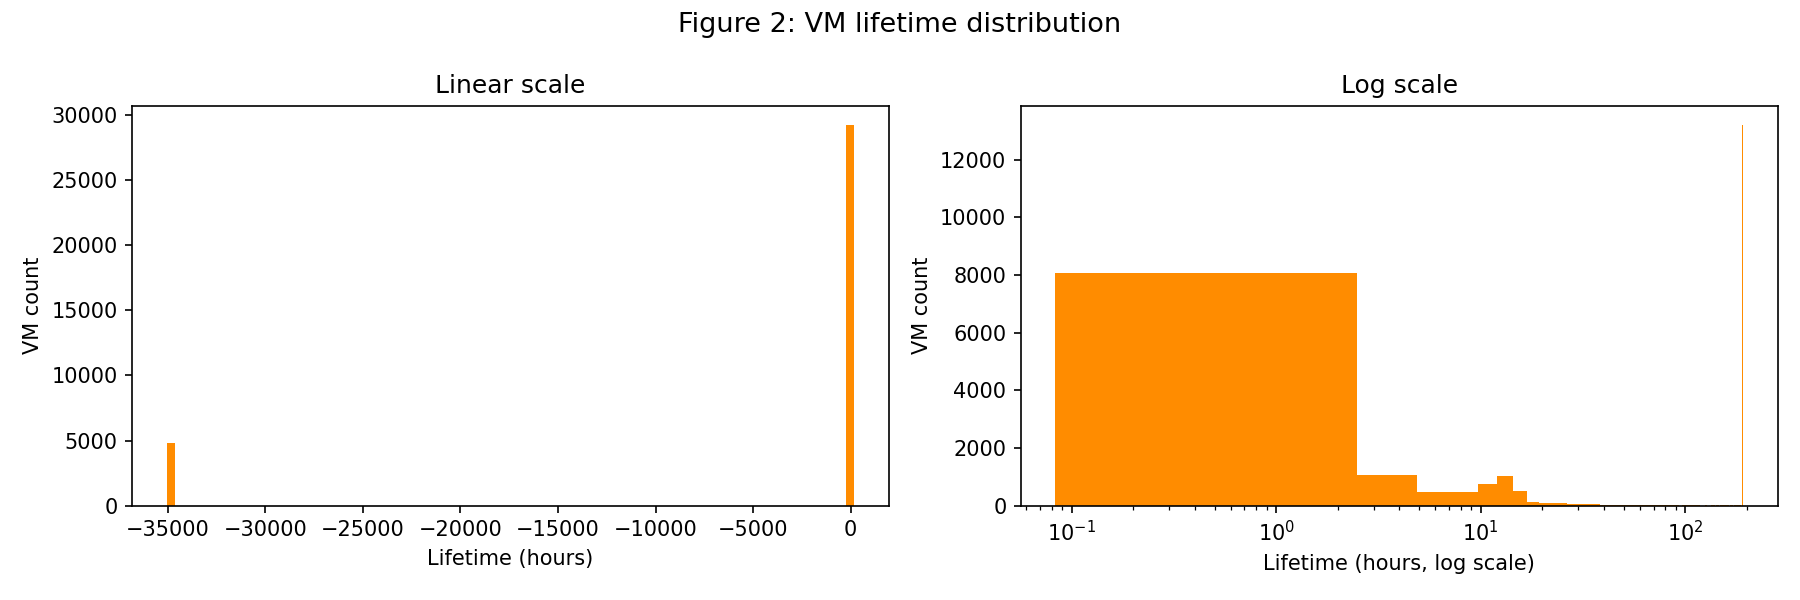
\includegraphics[width=\textwidth]{fig2_lifetimes.png}
  \caption{VM lifetime distribution for AMS20. Left: linear scale
  (negative lifetimes visible). Right: log scale of positive lifetimes
  only.}
\end{figure}

Approximately 14\% of VMs in AMS20 have \texttt{end\_time <
start\_time}, yielding negative computed lifetimes. Fig~D confirms
these all share a single negative depth of $\sim$35,000 hours,
corresponding to the default unset value
\texttt{end\_time = datetime(2020, 1, 1, 1, 1)} combined with a
\texttt{start\_time} in November 2023. A threshold filter of
\texttt{end\_time < datetime(2021, 1, 1)} cleanly identifies all
such VMs. Similarly, $\sim$6\% of VMs have zero lifetimes
(\texttt{start\_time == end\_time}).

All negative-lifetime VMs are caught by the HOTFIX filter
(\texttt{potentially NOT caught by HOTFIX: 0} across all ten traces),
so they do not corrupt the simulation. They must however be excluded
when computing statistics for augmentation parameter estimation.

\subsection{Data Quality Summary Across Traces}

\begin{center}
\begin{tabular}{lrrrrr}
\toprule
Trace & Total VMs & Neg. lifetime & Zero lifetime & Pos. lifetime & Spike VMs \\
\midrule
AMS20 & 34,029 & 14.1\% & 6.1\% & 79.8\% & 17.1\% \\
BLA   & 129,698 & 16.5\% & 6.1\% & 77.4\% & 11.4\% \\
BN9   & 178,224 & 15.5\% & 6.9\% & 77.6\% & 7.8\% \\
DSM   & 103,847 & 12.1\% & 7.7\% & 80.2\% & 10.4\% \\
DUB   & 79,151  & 10.6\% & 8.0\% & 81.5\% & 14.3\% \\
LON   & 23,450  & 15.1\% & 8.9\% & 76.0\% & 8.8\% \\
LVL   & 271,080 & 18.7\% & 14.3\% & 67.0\% & 3.4\% \\
SG2   & 141,018 & 16.9\% & 5.4\% & 77.6\% & 10.9\% \\
SYD   & 57,501  & 14.8\% & 4.3\% & 80.9\% & 11.8\% \\
YTO   & 80,280  & 19.5\% & 8.0\% & 72.5\% & 10.0\% \\
\bottomrule
\end{tabular}
\end{center}

``Spike VMs'' are those with \texttt{start\_time == trace\_min\_start},
i.e.\ VMs already running when trace collection began, whose arrival
time was set to the first tick of the trace window.

% =========================================================================
\section{Per-Node Statistics (Fig 3)}

\begin{figure}[H]
  \centering
  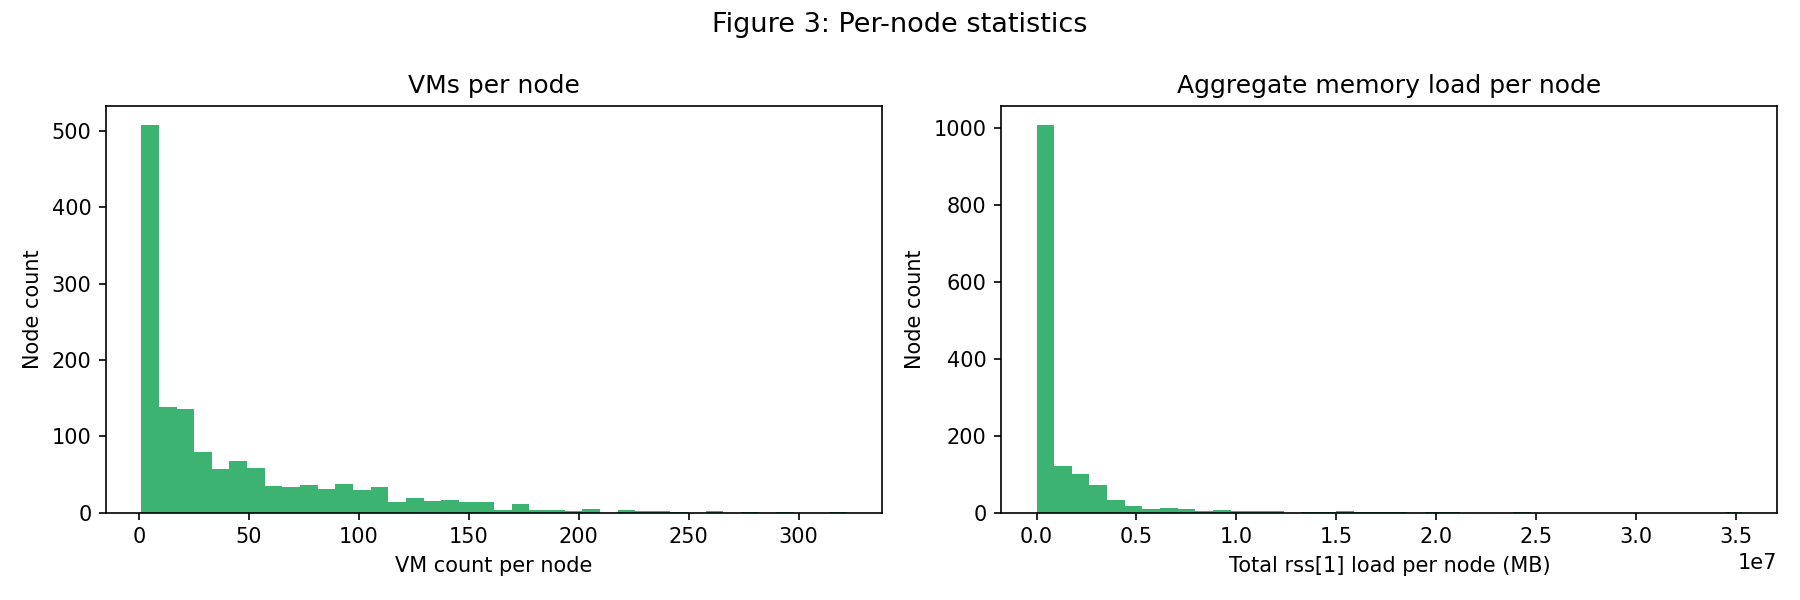
\includegraphics[width=\textwidth]{fig3_per_node.png}
  \caption{Per-node statistics for AMS20. Left: VM count per node.
  Right: aggregate \texttt{rss[1]} load per node.}
\end{figure}

Both distributions are right-skewed. The majority of nodes host fewer
than 20 VMs and carry modest aggregate load, while a small number of
nodes are substantially heavier. This heterogeneity means that pod
episode density varies considerably depending on which nodes are
sampled.

% =========================================================================
\section{VM Arrival Rate (Figs 4 and B)}

\begin{figure}[H]
  \centering
  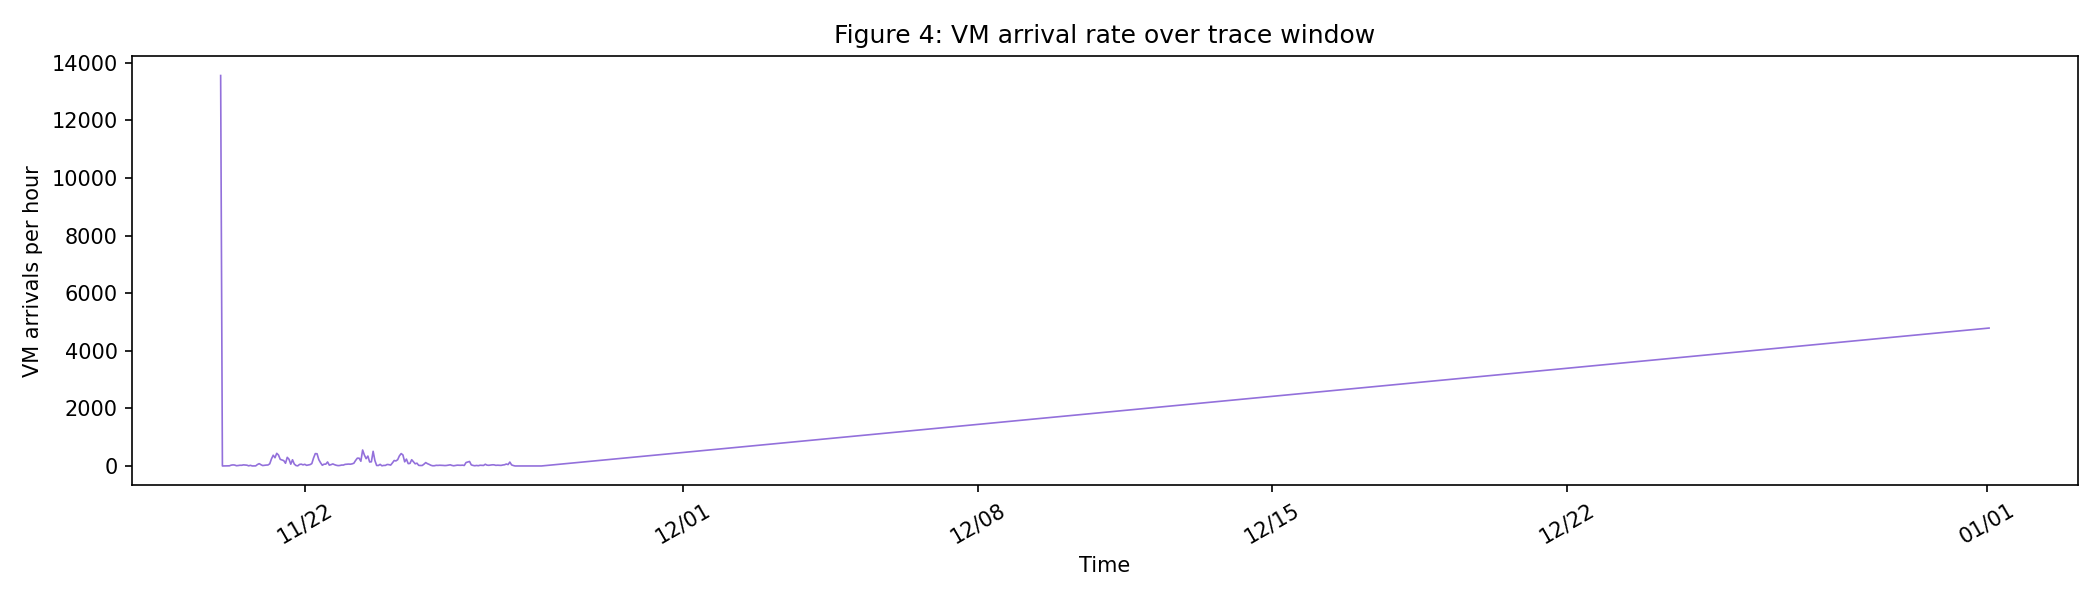
\includegraphics[width=\textwidth]{fig4_arrival_rate.png}
  \caption{Raw hourly VM arrival rate for AMS20. The large spike at
  trace start and apparent linear ramp are both artifacts (see text).}
\end{figure}

\begin{figure}[H]
  \centering
  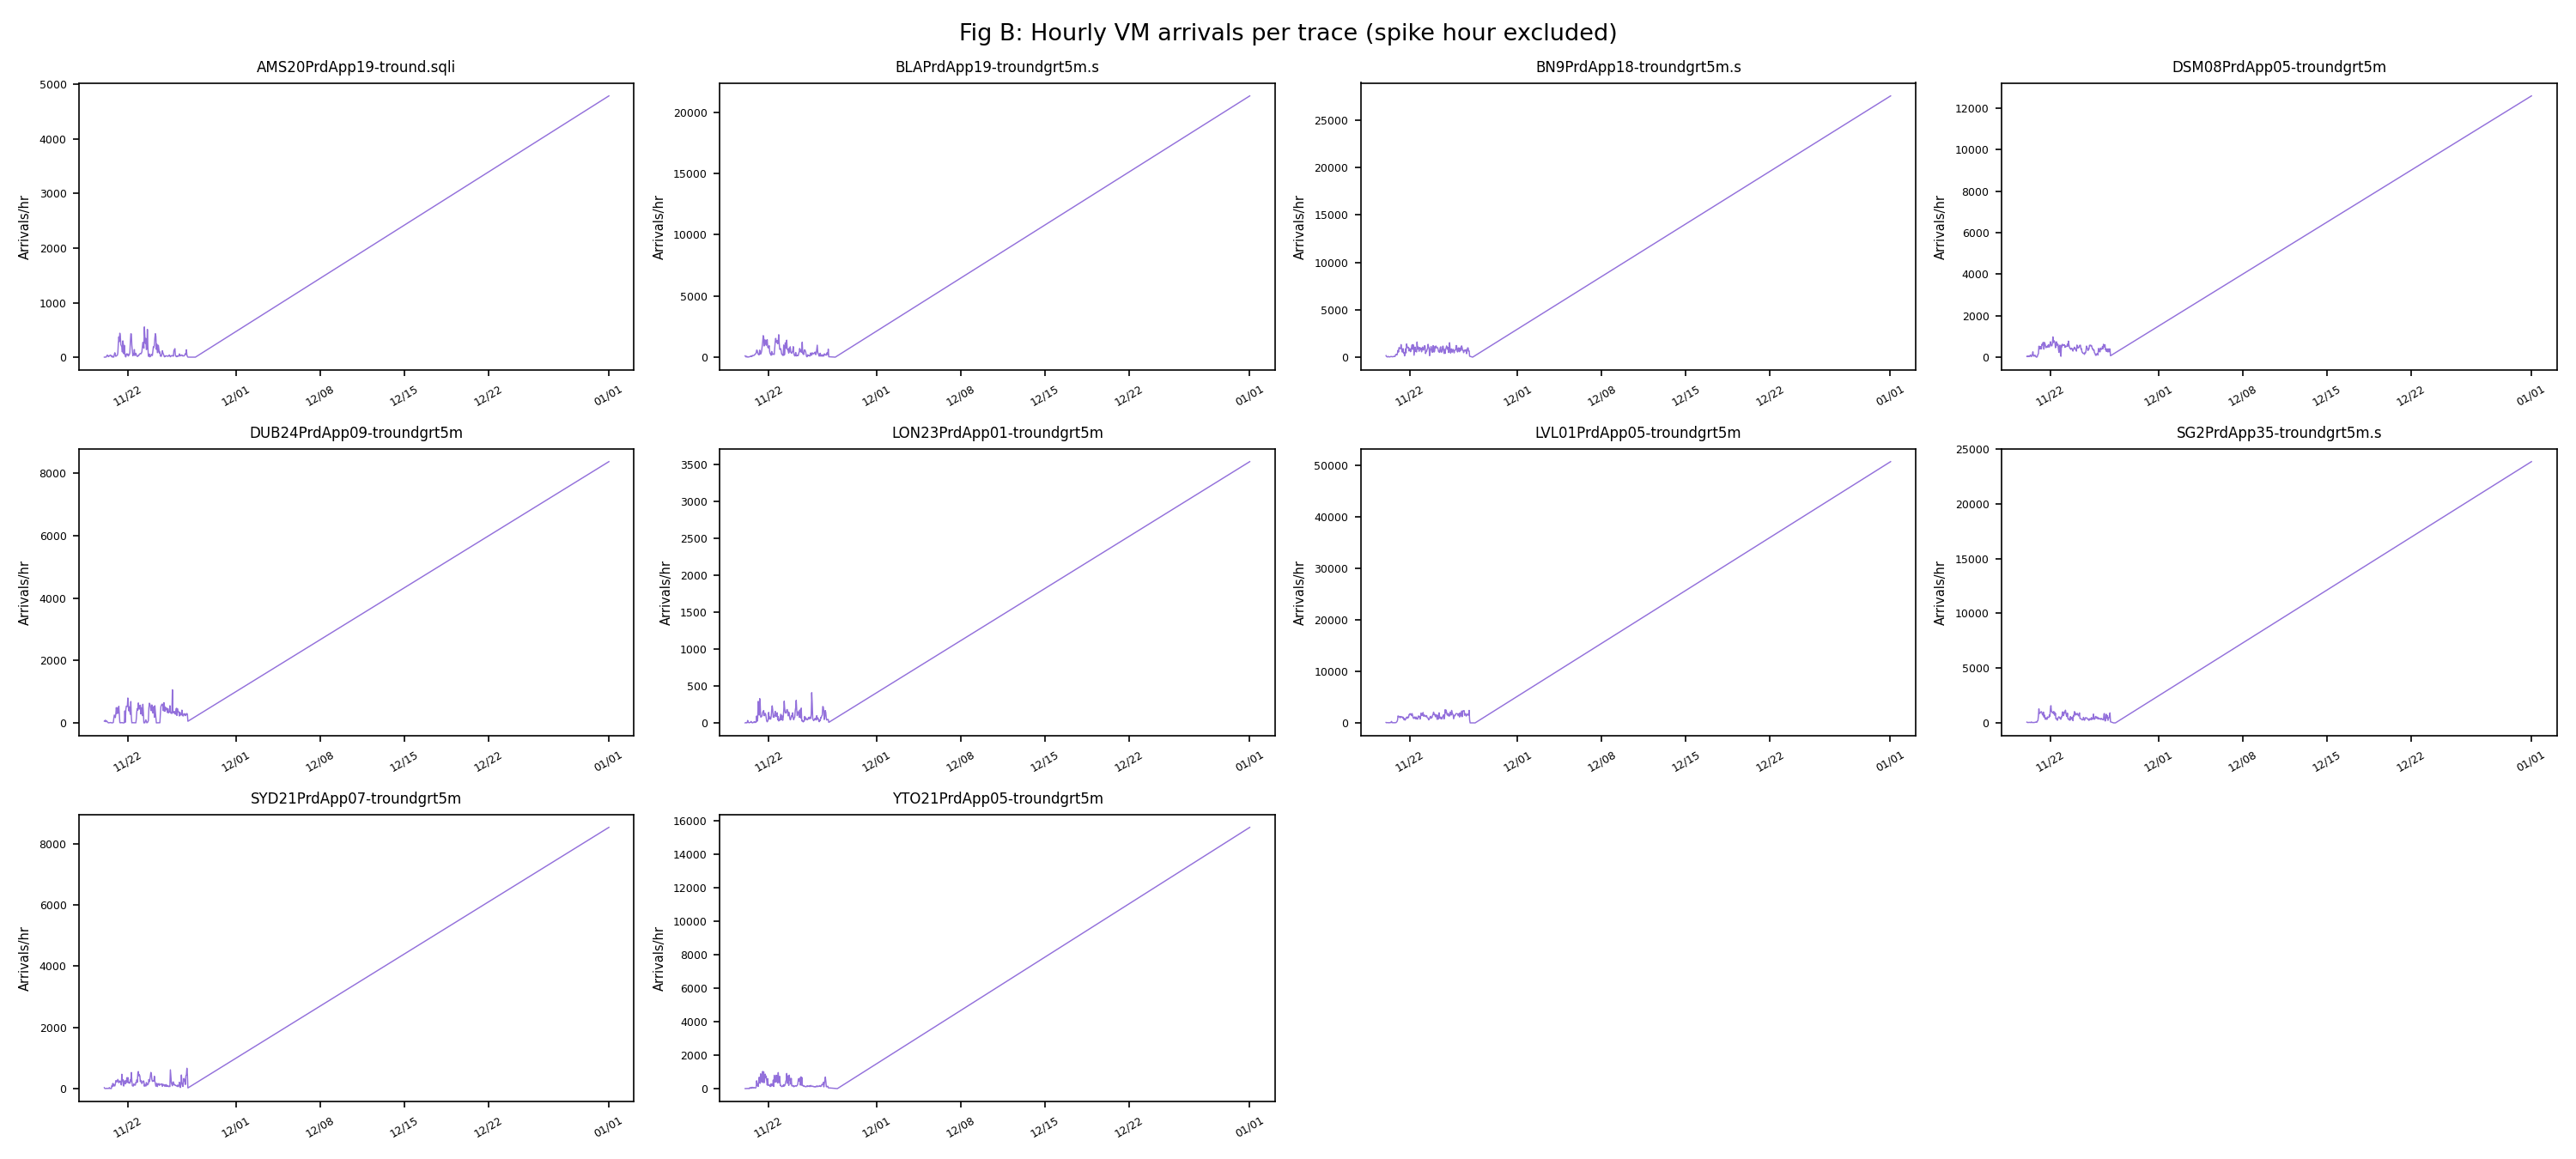
\includegraphics[width=\textwidth]{figB_arrival_rate_no_spike.png}
  \caption{Hourly VM arrivals per trace with the spike hour excluded.
  The linear ramp visible in Fig~4 is a matplotlib rendering artifact
  caused by a cluster of VMs with default \texttt{start\_time =
  datetime(2024, 1, 1, 1, 1)} binning to a distant future hour.}
\end{figure}

Two artifacts are present in the raw arrival rate plot:

\begin{enumerate}
  \item \textbf{Trace-start spike.} VMs already running at collection
  time are assigned \texttt{start\_time = trace\_min\_start}, creating
  a large artificial burst at the first tick (7--17\% of all VMs
  depending on trace). Fig~C confirms these spike VMs have the same
  \texttt{rss[1]} distribution as normal arrivals, so they are not a
  biased subsample.
  \item \textbf{Linear ramp.} VMs with the default
  \texttt{start\_time = datetime(2024, 1, 1, 1, 1)} bin to a single
  future hour far outside the trace window. matplotlib draws a straight
  line from the last real data point to that distant bin, producing the
  apparent ramp. The actual arrival signal (diurnal, with appropriate
  variation) is visible only in the left portion of Fig~4 and clearly
  in Fig~B after the spike hour is removed.
\end{enumerate}

% =========================================================================
\section{Negative Lifetime Deep-Dive (Figs D)}

\begin{figure}[H]
  \centering
  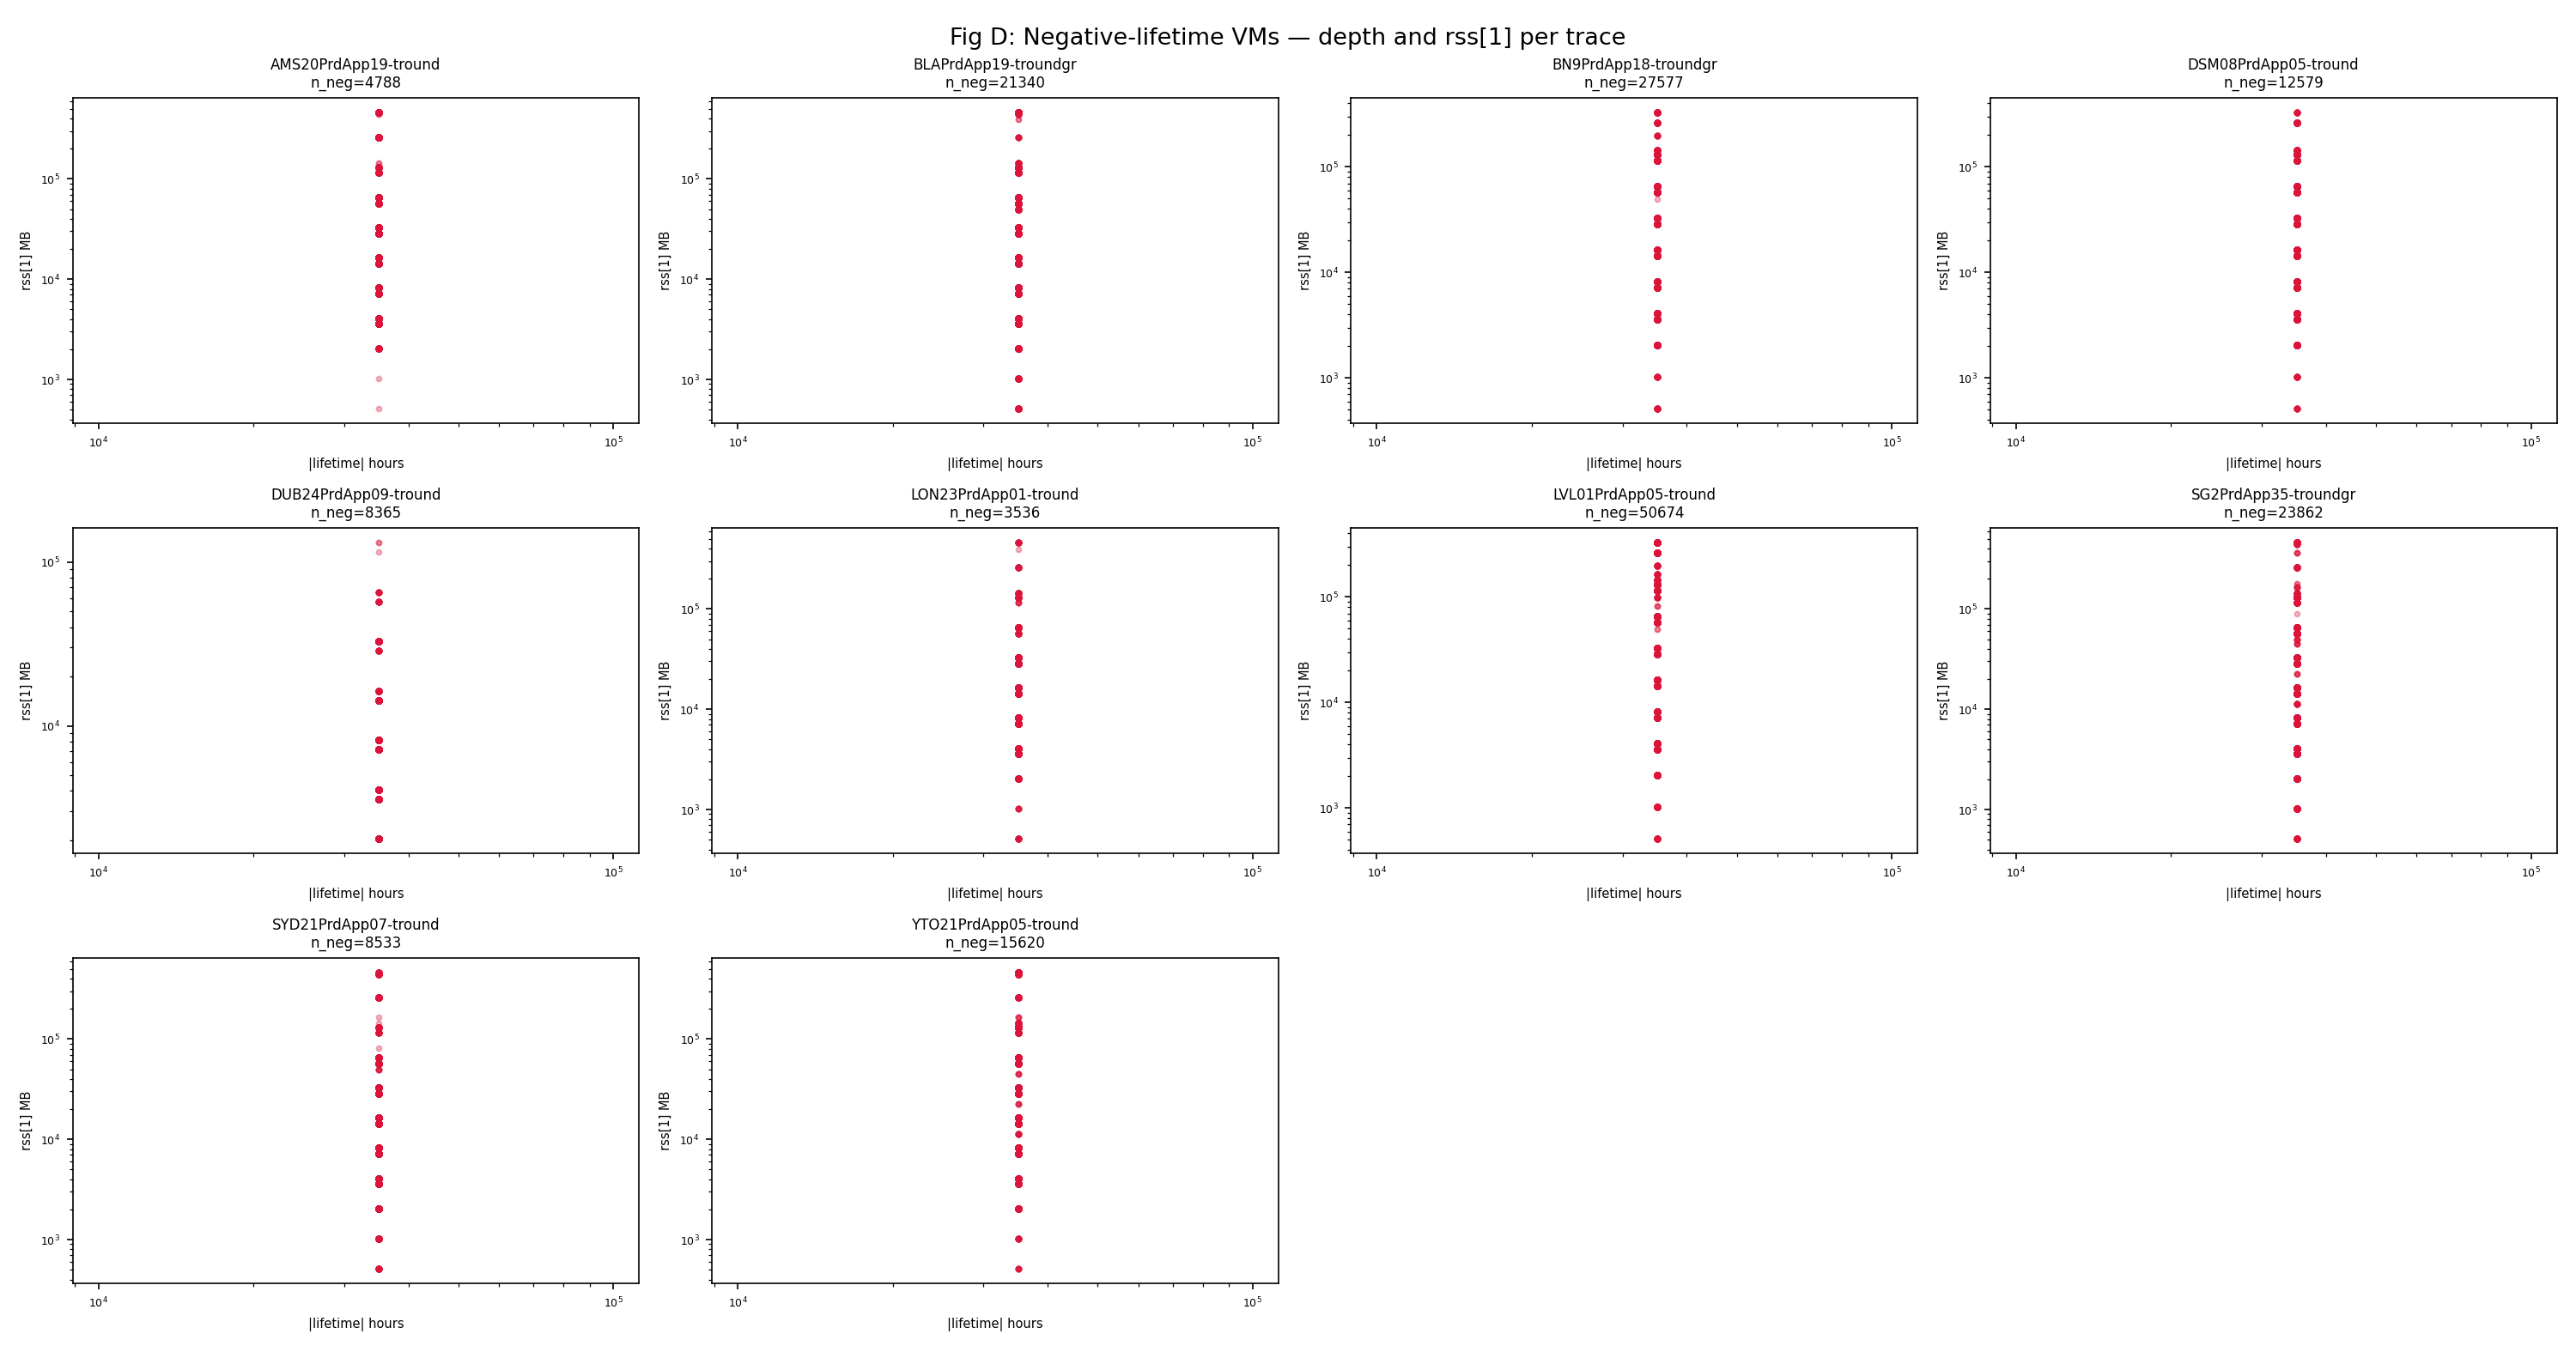
\includegraphics[width=\textwidth]{figD_negative_lifetimes_detail.png}
  \caption{Scatter of $|\text{lifetime}|$ vs \texttt{rss[1]} for
  negative-lifetime VMs per trace. All points cluster at a single
  x-value ($\sim$35,000--40,000 hours), confirming a single unset
  default rather than varied corruption.}
\end{figure}

All negative-lifetime VMs share the same negative depth regardless of
their \texttt{rss[1]}. The depth corresponds exactly to
\texttt{datetime(2020,1,1)} subtracted from a November 2023
\texttt{start\_time}. A single threshold suffices to identify them:
\texttt{end\_time < datetime(2021, 1, 1)}.

% =========================================================================
\section{HOTFIX Survival vs.\ Scale Factor (Fig 5)}

\begin{figure}[H]
  \centering
  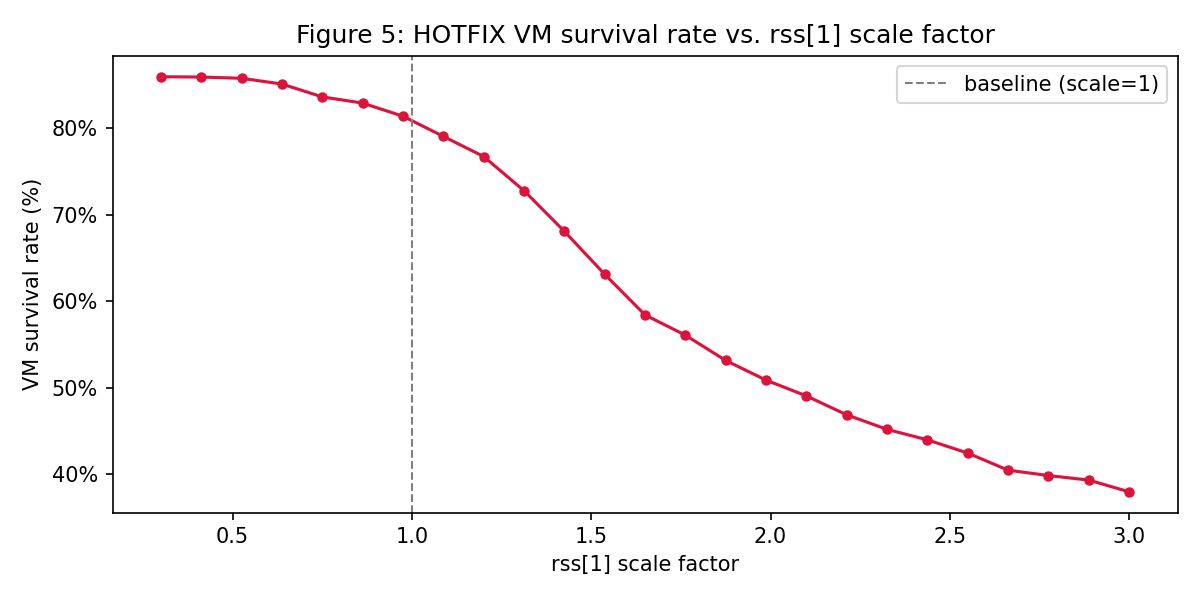
\includegraphics[width=0.75\textwidth]{fig5_hotfix_survival.png}
  \caption{Fraction of VMs surviving the HOTFIX filter as a function
  of episode-level \texttt{rss[1]} scale factor, computed across all
  nodes in AMS20.}
\end{figure}

At baseline (scale = 1.0), 81\% of VMs survive HOTFIX. The survival
curve is approximately flat below scale $\approx 0.7$ (floor of
$\sim$86\% imposed by VMs filtered for reasons other than DRAM
overflow) and drops steeply above scale $= 1.2$:

\begin{center}
\begin{tabular}{cc}
\toprule
Scale factor & Survival rate \\
\midrule
0.5  & 85.8\% \\
0.7  & 83.6\% \\
1.0  & 81.0\% \\
1.2  & 76.7\% \\
1.5  & 64.9\% \\
2.0  & 50.7\% \\
\bottomrule
\end{tabular}
\end{center}

\textbf{Design constraint:} episode-level scaling must remain in the
range $[0.7, 1.2]$ to avoid excessive VM dropout that would produce
unrepresentatively sparse training episodes.

% =========================================================================
\section{Episode Event Count Distribution (Figs E and F)}

\begin{figure}[H]
  \centering
  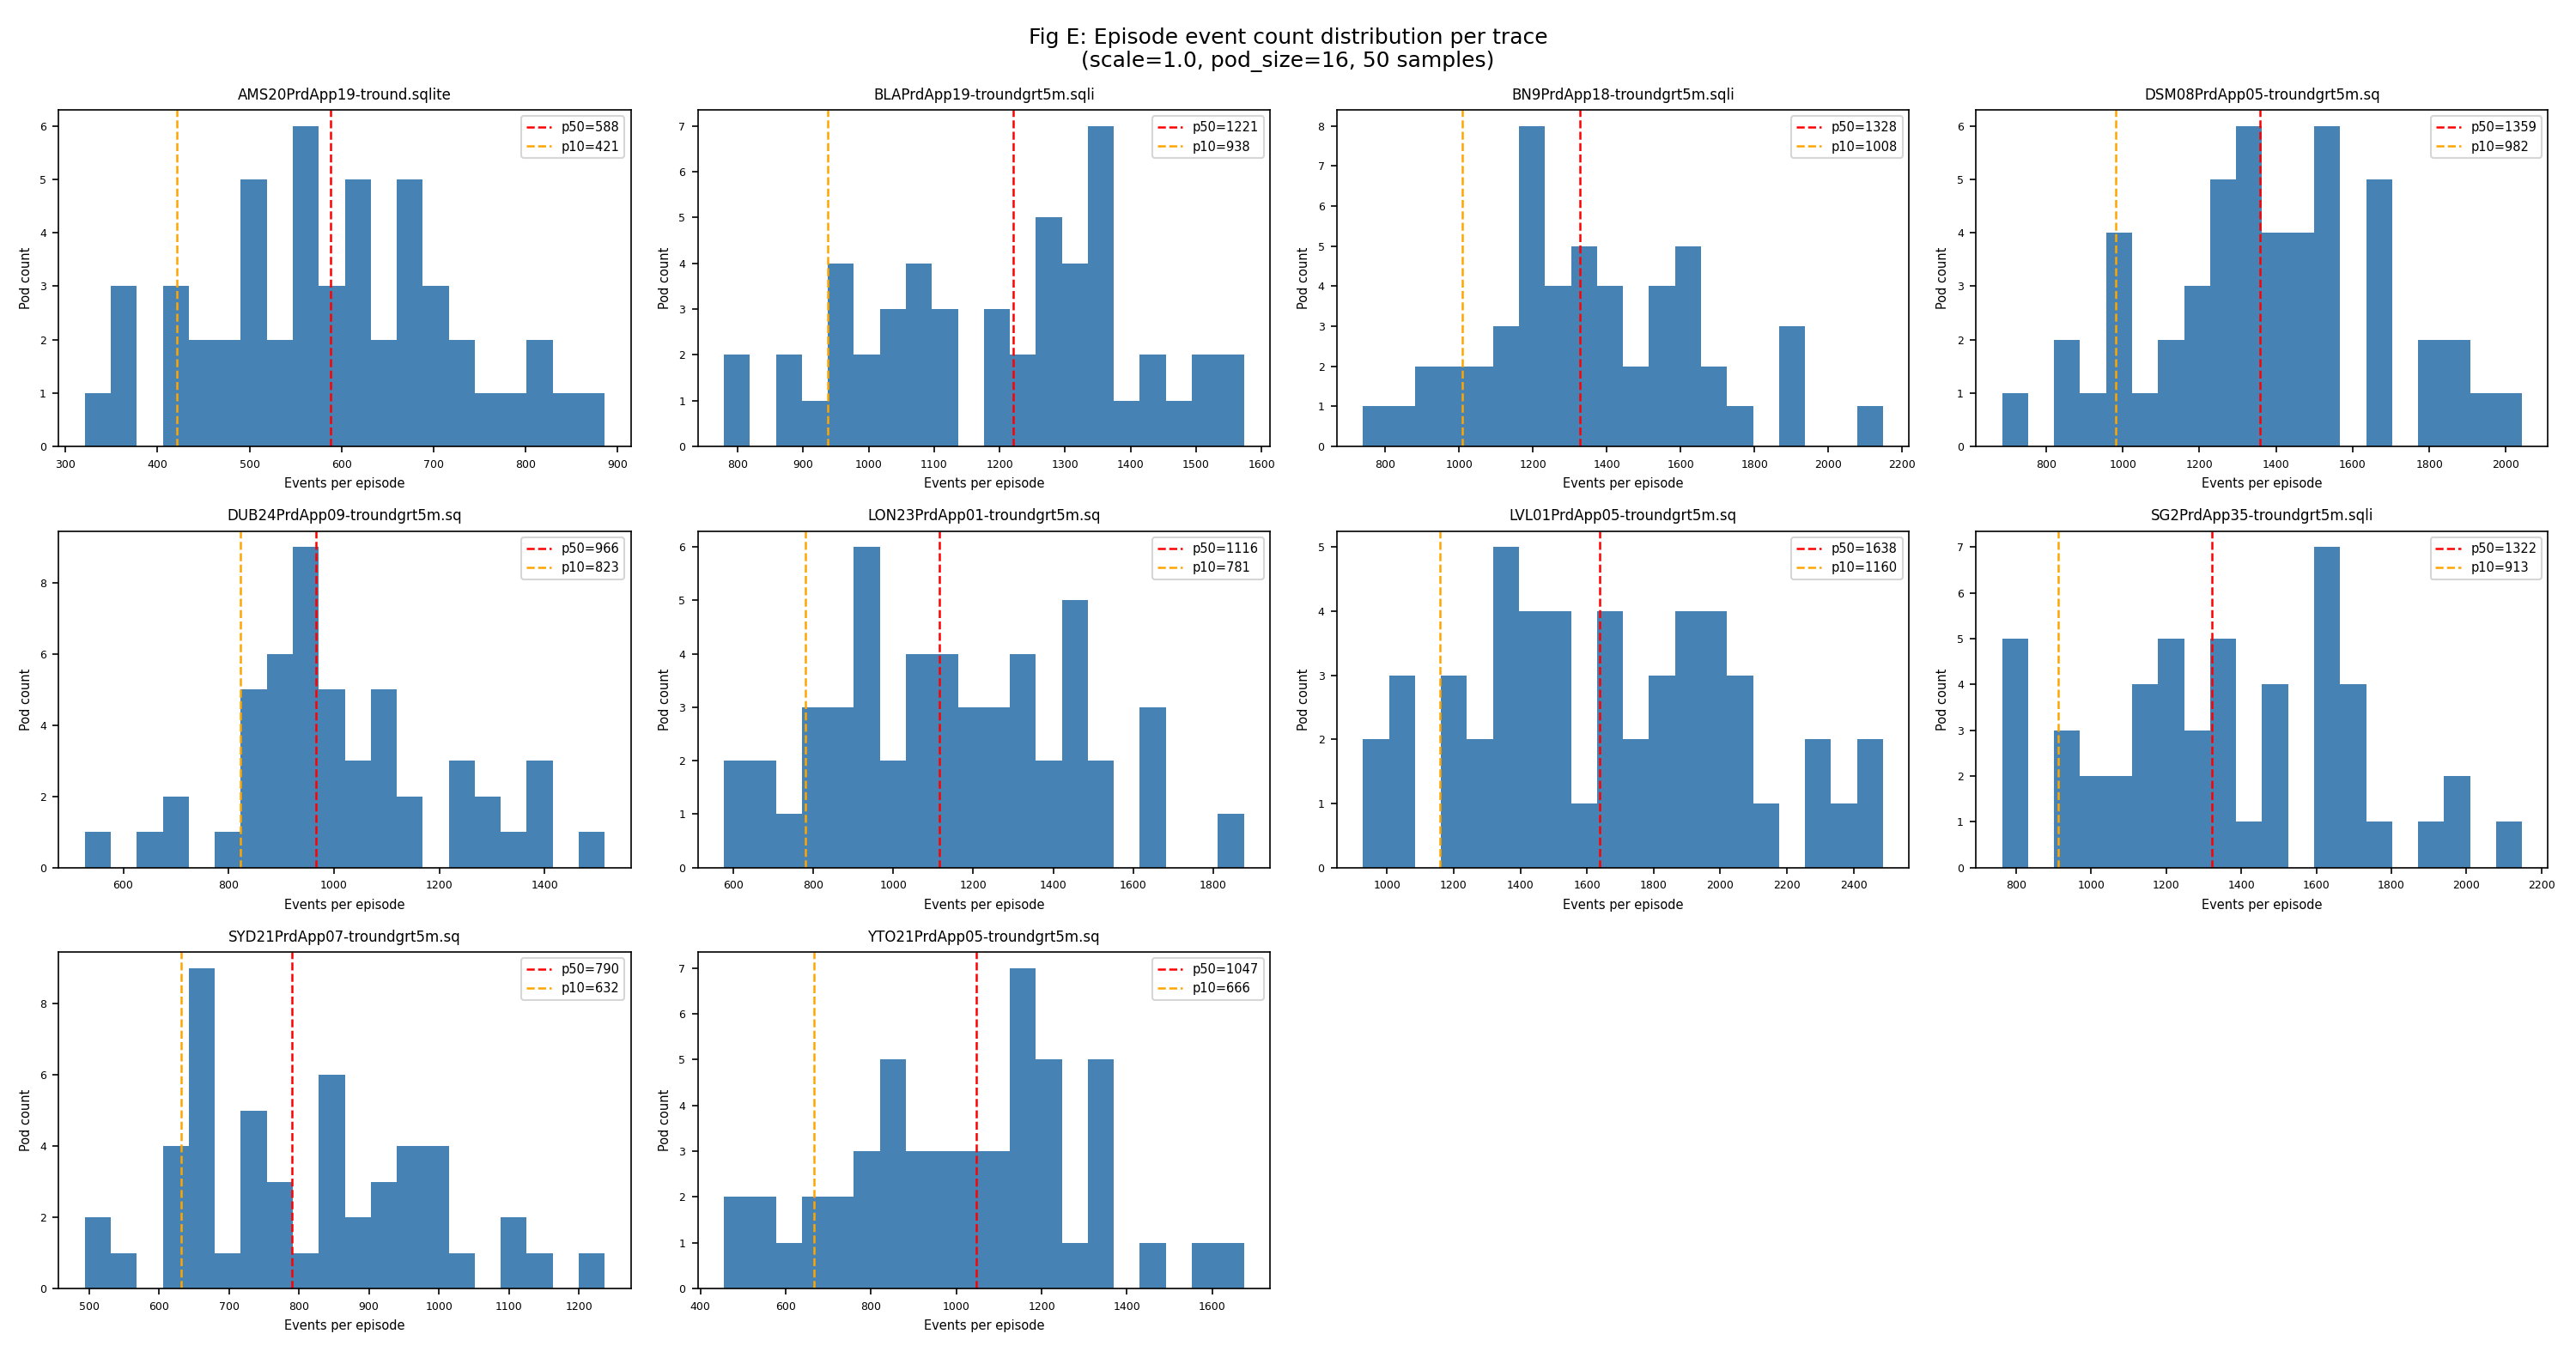
\includegraphics[width=\textwidth]{figE_event_counts.png}
  \caption{Distribution of events per episode across 50 random pod
  assignments per trace (scale=1.0, pod\_size=16). Red dashed: p50.
  Orange dashed: p10.}
\end{figure}

Episodes are dense. Across all ten traces, p10 ranges from
$\sim$400 to $\sim$1000 events per episode, and p50 ranges from
$\sim$590 to $\sim$1640. No trace produces near-empty episodes at
baseline, confirming that the bad-VM filtering (negative/zero
lifetimes) does not materially reduce episode signal.

\begin{center}
\begin{tabular}{lrr}
\toprule
Trace & p50 events & p10 events \\
\midrule
AMS20 & 588  & 421  \\
BLA   & 1221 & 938  \\
BN9   & 1328 & 1008 \\
DSM   & 1359 & 982  \\
DUB   & 966  & 823  \\
LON   & 1116 & 781  \\
LVL   & 1638 & 1160 \\
SG2   & 1322 & 913  \\
SYD   & 790  & 632  \\
YTO   & 1047 & 666  \\
\bottomrule
\end{tabular}
\end{center}

Given this density, the MIN\_EVENTS guard for augmentation can be set
conservatively at 100 events per episode; in practice it will almost
never trigger within the safe scaling range of $[0.7, 1.2]$.

% =========================================================================
\section{Other rss Fields (Fig 6)}

\begin{figure}[H]
  \centering
  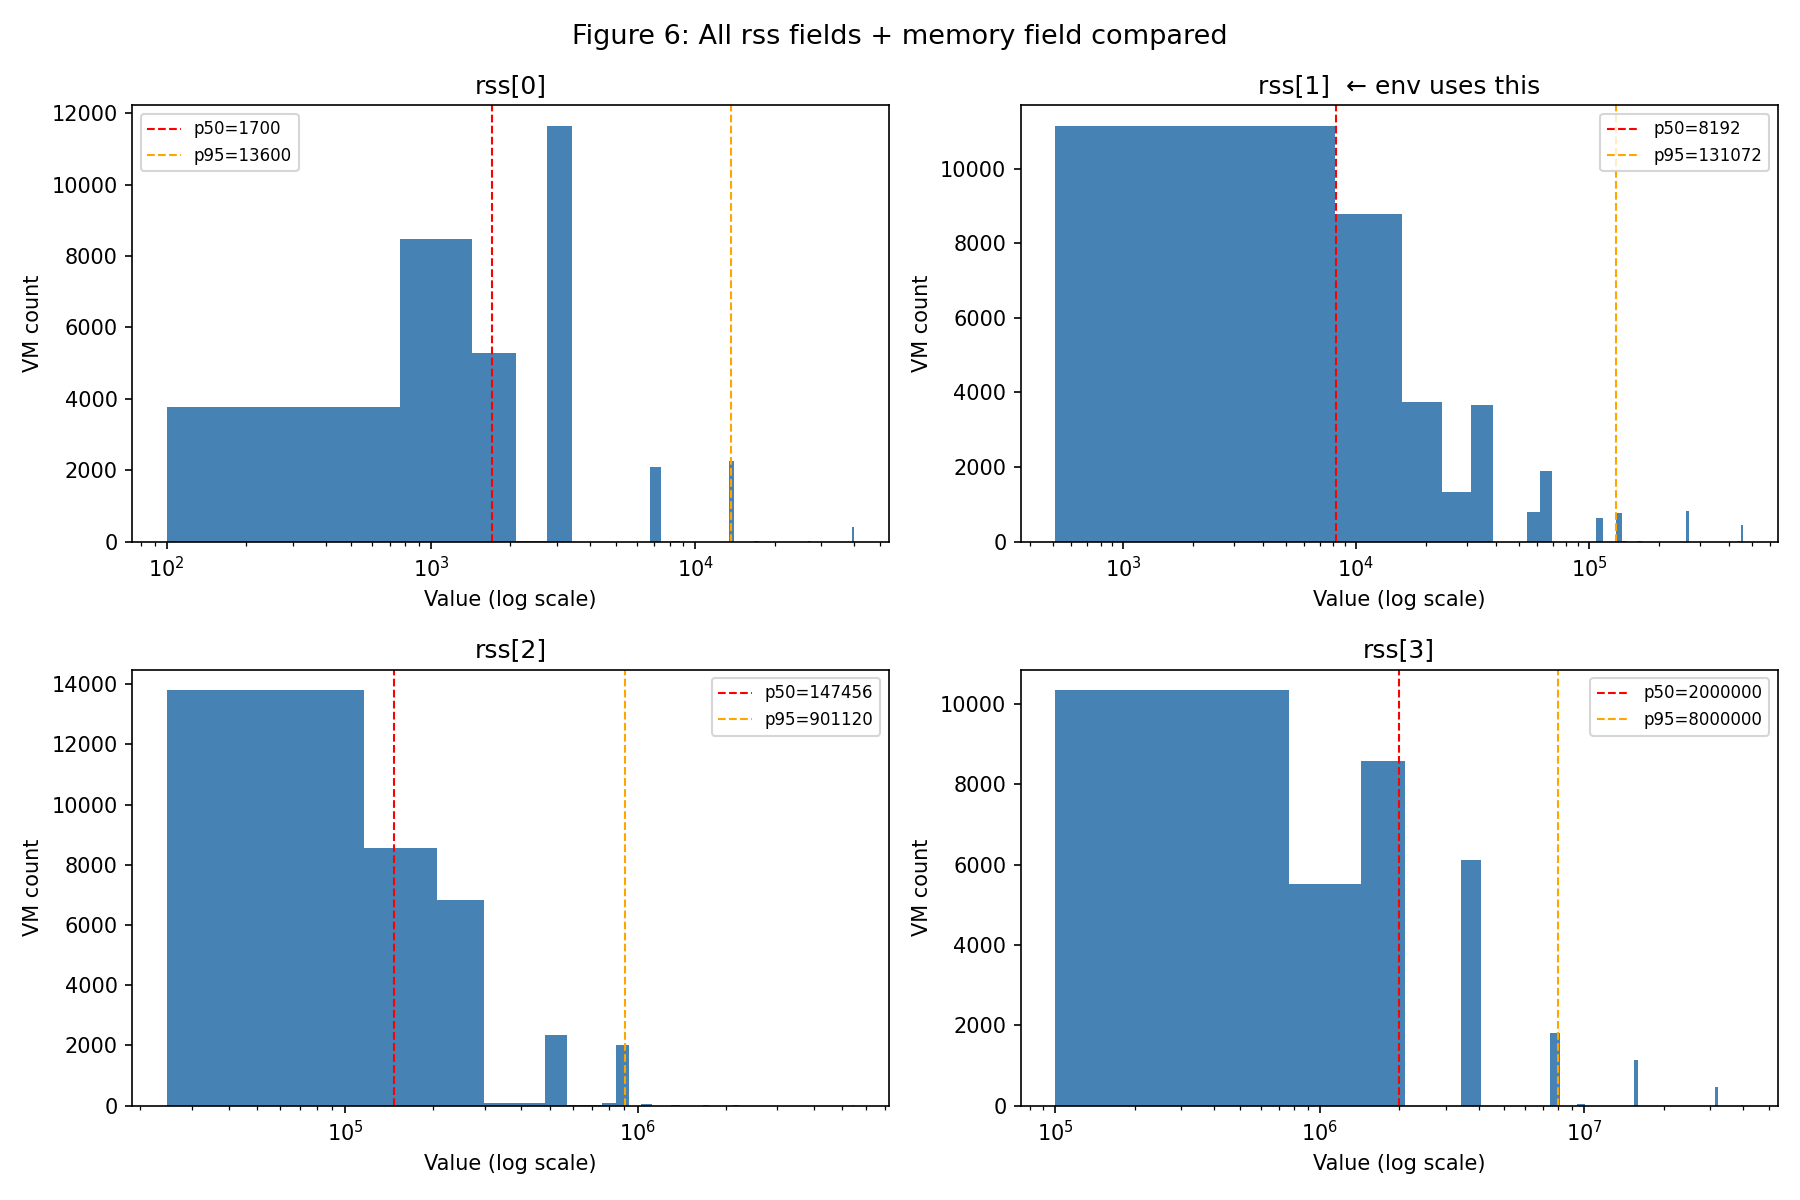
\includegraphics[width=\textwidth]{fig6_rss_fields.png}
  \caption{Distributions of all four \texttt{rss} fields (log scale)
  for AMS20. \texttt{rss[1]} is the only field used by the env.}
\end{figure}

\begin{center}
\begin{tabular}{lrrl}
\toprule
Field & p50 & p95 & Likely interpretation \\
\midrule
\texttt{rss[0]} & 1,700      & 13,600      & vCPU allocation (scaled) \\
\texttt{rss[1]} & 8,192      & 131,072     & Memory (MB) — used by env \\
\texttt{rss[2]} & 147,456    & 901,120     & Storage (MB) \\
\texttt{rss[3]} & 2,000,000  & 8,000,000   & Network bandwidth or IOPS \\
\bottomrule
\end{tabular}
\end{center}

None of the other fields are a viable substitute for \texttt{rss[1]}
as a memory demand signal. The \texttt{avg\_mem\_ts} time series
(utilisation percentages against \texttt{rss[1]}) would provide a
richer dynamic demand signal but requires env changes to consume.

% =========================================================================
\section{Data Augmentation Design}
\label{sec:augmentation}

The augmentation strategy should follow the same principle used in
high-throughput physics simulation systems: generate new training
episodes by randomizing environment conditions, rather than perturbing
individual samples in unrealistic ways. In this project, the correct
unit of randomization is the \textbf{episode}, not the VM.

\subsection{Why Episode-Level Augmentation}

Fig~1 shows that \texttt{rss[1]} is a discrete SKU-like variable
(powers-of-two clusters). Per-VM scaling would create synthetic memory
sizes that do not exist in production and would break the empirical VM
type structure. Therefore, each augmented episode applies a single
global factor to all VM memory requests:
\[
\texttt{rss[1]}^\prime = s \cdot \texttt{rss[1]}, \qquad
s \sim \mathcal{U}(0.7, 1.2).
\]
The safe range $[0.7, 1.2]$ is dictated by HOTFIX survival
(Fig~5): lower values provide little additional variation, while higher
values cause severe VM dropout and produce unrealistically sparse
episodes.

\subsection{Augmentation Knobs}

For each training episode, sample an augmentation configuration:
\begin{enumerate}
  \item \textbf{Trace ID} from the 10-trace corpus (uniform or weighted).
  \item \textbf{Pod seed} (node subset sampling), already supported by
  current reset logic.
  \item \textbf{Memory scale} $s \in [0.7,1.2]$ applied uniformly to all
  VM \texttt{rss[1]} in that episode.
  \item \textbf{Optional arrival jitter} (small bounded tick shifts) to
  decorrelate exact co-arrivals while preserving chronology.
  \item \textbf{Optional lifetime perturbation} for valid positive-lifetime
  VMs only (never applied to known invalid default timestamps).
  \item \textbf{Optional topology perturbation} via low-rate random edge
  removal (failure injection), e.g.\ 1--5\% link failures per episode.
\end{enumerate}

This is analogous to domain randomization in simulator-based RL: each
episode represents a different, but still plausible, operating regime.

\subsection{Validity Guards}

Each augmented episode must satisfy:
\begin{itemize}
  \item \textbf{HOTFIX feasibility}: apply the same HOTFIX filter after
  augmentation.
  \item \textbf{Minimum density}: enforce \texttt{MIN\_EVENTS} = 100.
  \item \textbf{Data quality}: exclude negative-lifetime default artifacts
  from any augmentation parameter estimation.
  \item \textbf{Topology safety}: reject samples that disconnect hosts from
  all MPDs; cap failure injection to the graceful-degradation regime
  (recommended $\leq 5\%$).
\end{itemize}

If a sampled configuration fails the guards, resample augmentation
parameters for that episode.

\subsection{Recommended Sampling Policy}

To avoid over-concentrating around the baseline:
\begin{itemize}
  \item Sample $s$ from a clipped triangular distribution centered at 1.0
  with support $[0.7,1.2]$ for stable yet diverse coverage.
  \item Use mixed-trace batches so each training window sees both
  low-utilization and high-utilization datacenter regimes.
  \item Stratify pod seeds to avoid repeatedly sampling the same easy pods.
\end{itemize}

\subsection{Expected Effect on RL Training}

Episode-level augmentation increases the diversity of load trajectories
without violating SKU structure, improves robustness to cluster-to-cluster
and time-to-time demand shifts, and reduces overfitting to a single
pod/trace configuration. Most importantly, it preserves simulator
mechanics (HOTFIX, event ordering, topology constraints), so policy
improvements transfer to non-augmented evaluation runs.

\subsection{Implementation Sketch (Pseudocode)}

\begin{verbatim}
def sample_episode_config(rng):
    trace_id = sample_trace(rng)                 # one of 10 traces
    pod_seed = rng.randint(0, 2**31 - 1)         # controls pod node mapping
    scale = sample_triangular(rng, lo=0.7, mode=1.0, hi=1.2)
    arrival_jitter = rng.choice([0, 0, 1])       # optional, small
    lifetime_noise = rng.choice([0.0, 0.0, 0.05])# optional, mild
    fail_ratio = rng.choice([0.0, 0.0, 0.01, 0.02, 0.03, 0.05])  # optional
    return {
        "trace_id": trace_id,
        "pod_seed": pod_seed,
        "scale": scale,
        "arrival_jitter": arrival_jitter,
        "lifetime_noise": lifetime_noise,
        "fail_ratio": fail_ratio,
    }

def build_augmented_episode(cfg):
    events = load_events(cfg["trace_id"], pod_seed=cfg["pod_seed"])
    topo = inject_link_failures(base_topology, ratio=cfg["fail_ratio"])
    if not host_connectivity_ok(topo):                    # at least 1 MPD/host
        return None
    events = scale_memory(events, factor=cfg["scale"])  # rss[1] only
    events = jitter_arrivals(events, max_shift=cfg["arrival_jitter"])
    events = perturb_lifetimes(events, frac=cfg["lifetime_noise"],
                               positive_only=True)
    events = apply_hotfix(events)                        # required
    if len(events) < 100:                               # MIN_EVENTS guard
        return None
    return events
\end{verbatim}

In practice, training loop integration is:
\begin{enumerate}
  \item sample config at \texttt{env.reset()},
  \item construct episode events with the augmented pipeline,
  \item resample if guards fail,
  \item run rollout and log config metadata with rewards/savings.
\end{enumerate}

\end{document}